\documentclass[tikz,border=6pt]{standalone}
\usepackage{xcolor}
\usetikzlibrary{arrows.meta,decorations.pathmorphing,calc,positioning,fit,backgrounds,shapes.geometric}
\definecolor{red}{HTML}{A50F2D}\definecolor{ink}{HTML}{141414}\definecolor{gry}{HTML}{5F5F5F}\definecolor{lgry}{HTML}{E6E6E6}
\definecolor{blu}{HTML}{2B6CB0}\definecolor{teal}{HTML}{1B9E8F}\definecolor{org}{HTML}{E8702A}\definecolor{grn}{HTML}{2E9E5B}\definecolor{mag}{HTML}{D81B60}\definecolor{pur}{HTML}{5B2C83}
\tikzset{fibre/.style={ink,line width=1.6pt,line cap=round},
 sis1/.style={org,line width=1.8pt,line cap=round},sis2/.style={blu,line width=1.8pt,line cap=round},
 lab/.style={font=\sffamily\small,text=ink},lbl/.style={font=\sffamily\footnotesize,text=gry,align=center},ttl/.style={font=\sffamily\bfseries\small,text=ink},
 ctcf/.style={-{Triangle[length=5pt,width=6pt]},pur,line width=2.4pt},
 cohesin/.style={grn,line width=1.6pt}}

% ---- shared drawing macros: a DNA duplex is a dark tube with a light core
\newcommand{\dx}[2][ink]{\draw[line width=3.6pt,#1,line cap=round] #2; \draw[line width=1.3pt,white,line cap=round] #2;}
% omega-shaped loop: base at (x,y), radius r
\newcommand{\omegapath}[3]{(#1-0.35,#2) .. controls (#1-0.35,#2+0.45) and (#1-#3,#2+0.35) .. (#1-#3,#2+#3+0.45) arc[start angle=180,end angle=0,radius=#3] .. controls (#1+#3,#2+0.35) and (#1+0.35,#2+0.45) .. (#1+0.35,#2)}
% replication eye: origin at (x,y), half width w, half height h
\newcommand{\eyetop}[4]{(#1-#3,#2) .. controls (#1-#3*0.5,#2+#4*1.33) and (#1+#3*0.5,#2+#4*1.33) .. (#1+#3,#2)}
\newcommand{\eyebot}[4]{(#1-#3,#2) .. controls (#1-#3*0.5,#2-#4*1.33) and (#1+#3*0.5,#2-#4*1.33) .. (#1+#3,#2)}
\newcommand{\eye}[4]{\dx[org]{\eyetop{#1}{#2}{#3}{#4}}\dx[blu]{\eyebot{#1}{#2}{#3}{#4}}\fill[teal] (#1-#3,#2) circle (3.2pt) (#1+#3,#2) circle (3.2pt);}
\newcommand{\ring}[3]{\draw[grn,line width=1.8pt] (#1,#2) ellipse (#3 and #3*1.35);}
\newcommand{\gseg}[3]{\dx[gry]{(#2,#1) -- (#3,#1)}}

\begin{document}
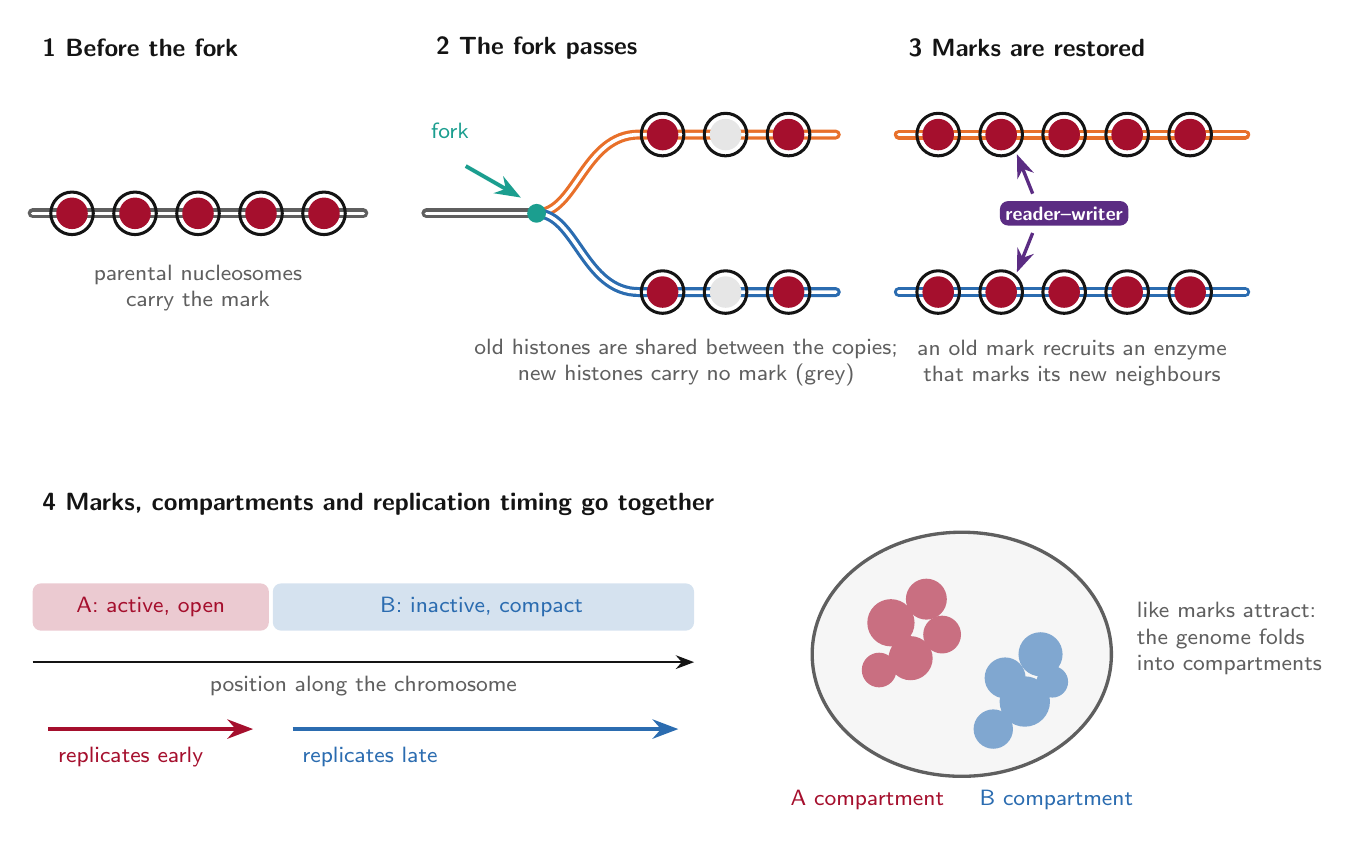
\begin{tikzpicture}[font=\sffamily\small,>=Stealth]
% nucleosome: histone disc with DNA wrapped around it
\newcommand{\nuc}[3]{\draw[ink,line width=1.1pt] (#1,#2) circle (0.27); \fill[#3] (#1,#2) circle (0.2);}
\node[ttl,anchor=west] at (0,3.6) {1  Before the fork};  \node[ttl,anchor=west] at (5.0,3.6) {2  The fork passes};  \node[ttl,anchor=west] at (11.0,3.6) {3  Marks are restored};
% 1 parental duplex with marked nucleosomes
\dx[gry]{(0,1.5) -- (4.2,1.5)} \foreach \x in {0.5,1.3,2.1,2.9,3.7}{\nuc{\x}{1.5}{red}}
\node[lbl] at (2.1,0.55) {parental nucleosomes\\ carry the mark};
% 2 replication fork: parental DNA splits into two daughters
\dx[gry]{(5.0,1.5) -- (6.4,1.5)}
\dx[org]{(6.4,1.5) .. controls (6.9,1.5) and (7.0,2.5) .. (7.7,2.5) -- (10.2,2.5)}
\dx[blu]{(6.4,1.5) .. controls (6.9,1.5) and (7.0,0.5) .. (7.7,0.5) -- (10.2,0.5)}
\fill[teal] (6.4,1.5) circle (3.4pt); \draw[->,teal,line width=1.4pt] (5.5,2.1) -- (6.2,1.7);
\node[lbl,teal] at (5.3,2.55) {fork};
\foreach \x/\c in {8.0/red,8.8/lgry,9.6/red}{\nuc{\x}{2.5}{\c}\nuc{\x}{0.5}{\c}}
\node[lbl] at (8.3,-0.4) {old histones are shared between the copies;\\ new histones carry no mark (grey)};
% 3 restored
\dx[org]{(11.0,2.5) -- (15.4,2.5)} \dx[blu]{(11.0,0.5) -- (15.4,0.5)}
\foreach \x in {11.5,12.3,13.1,13.9,14.7}{\nuc{\x}{2.5}{red}\nuc{\x}{0.5}{red}}
\node[fill=pur,rounded corners=3pt,text=white,font=\sffamily\bfseries\scriptsize,inner sep=2pt] at (13.1,1.5) {reader--writer};
\draw[->,pur,line width=1.2pt] (12.7,1.75) -- (12.5,2.25); \draw[->,pur,line width=1.2pt] (12.7,1.25) -- (12.5,0.75);
\node[lbl] at (13.2,-0.4) {an old mark recruits an enzyme\\ that marks its new neighbours};
% row 2
\begin{scope}[yshift=-5.4cm]
\node[ttl,anchor=west] at (0,3.2) {4  Marks, compartments and replication timing go together};
\fill[red!22,rounded corners=3pt] (0,1.6) rectangle (3.0,2.2); \fill[blu!20,rounded corners=3pt] (3.05,1.6) rectangle (8.4,2.2);
\node[lbl,red] at (1.5,1.9) {A: active, open}; \node[lbl,blu] at (5.7,1.9) {B: inactive, compact};
\draw[->,ink,thick] (0,1.2) -- (8.4,1.2); \node[lbl] at (4.2,0.9) {position along the chromosome};
\draw[->,red,line width=1.4pt] (0.2,0.35) -- (2.8,0.35); \node[lbl,red,anchor=west] at (0.2,0.0) {replicates early};
\draw[->,blu,line width=1.4pt] (3.3,0.35) -- (8.2,0.35); \node[lbl,blu,anchor=west] at (3.3,0.0) {replicates late};
% nucleus with two clusters
\draw[gry,line width=1.2pt,fill=lgry!35] (11.8,1.3) circle (1.9 and 1.55);
\foreach \x/\y/\r in {10.9/1.7/0.3,11.35/2.0/0.26,11.15/1.25/0.28,10.75/1.1/0.22,11.55/1.55/0.24}{\fill[red!60] (\x,\y) circle (\r);}
\foreach \x/\y/\r in {12.6/0.7/0.32,12.2/0.35/0.25,12.8/1.3/0.28,12.35/1.0/0.26,12.95/0.95/0.2}{\fill[blu!60] (\x,\y) circle (\r);}
\node[lbl,red] at (10.6,-0.55) {A compartment}; \node[lbl,blu] at (13.0,-0.55) {B compartment};
\node[lbl,align=left,anchor=west] at (13.9,1.5) {like marks attract:\\ the genome folds\\ into compartments};
\end{scope}
\end{tikzpicture}
\end{document}
